\documentclass[12pt, a4paper]{article}
\usepackage[utf8]{inputenc}
\usepackage[russian]{babel}
\usepackage{cmap}
\usepackage{amsmath}
\usepackage{amsfonts}
\usepackage{amssymb}
\usepackage{makeidx}
\usepackage{graphicx}
\usepackage{hyperref}
\usepackage{makecell}
\usepackage[table]{xcolor}
\usepackage{verbatim}

\newcommand{\ci}[1]{\indent\texttt{#1} \\}
\newcommand{\cn}[1]{\noindent\texttt{#1} \\}
\newcommand{\cci}[2]{\indent\texttt{#1\indent \#} - #2 \\}
\newcommand{\ccn}[2]{\noindent\texttt{#1\indent \#} - #2 \\}
\newcommand{\tc}[2]{\noindent #2 \\ \indent\texttt{#1} \\}

\begin{document}
	
	\begin{center} {\Huge Nets} \end{center}

	\section{Полезные ссылки}
	\begin{itemize}
		\item \href{https://habr.com/ru/articles/794262/}{Создаём виртуальную сеть, как это делает Docker}
		\item \href{https://developers.redhat.com/blog/2018/10/22/introduction-to-linux-interfaces-for-virtual-networking}{Introduction to Linux interfaces for virtual networking}
	\end{itemize}
	
	\section{Управление линками}
	\ccn{\# ip link add <name> type <type>}{добавить link с типом type}
	\ccn{\# ip link delete <name>}{удалить link}
	\ccn{\# ip link set <name> [up|down]}{включить / выключить}
	\ccn{\# ip link set <name> master <bridge>}{добавить link в bridge}

	\section{Адреса}
	\ccn{\# ip addr add 127.0.0.1/8 dev lo}{задать адрес}
	
	\section{route}
	\tc{\# ip route add default via 10.100.0.1}{Задать маршрут по умолчанию:}
	
	\section{Info}
	\ccn{\$ netstat -tulpen}{Открытые порты}
	
	\section{Namespaces}
	\ccn{\# ip netns add <name>}{добавить новый namespace}
	\ccn{\# ip netns list}{список namespaces}
	\ccn{\# ip -n <name> a}{список сетевых устройств в namespace}
	\tc{\# ip -n <name> addr add 127.0.0.1/8 dev lo}{Задать адрес сетевому устройству в namespace:}
	\tc{\# ip netns exec <name> python3 -m http.server}{Запускаем http-сервер в рамках нового netns:}
	
	\section{System}
	\tc{\# sysctl -w net.ipv4.ip\_forward=1}{Перенаправлять трафик между интерфейсами:}
	\tc{\# sysctl -w net.ipv4.conf.<name>.route\_localnet=1}{Разрешает перенаправления трафика на локальные сети:}
	
	
	
	

	%\tableofcontents
	
	%\section{Введение}

\subsection{Требования к ядру}
Рекомендуется использовать ядро Linux 4.9 (релиз в декабре 2016 года) или более
новое. Некоторые параметры конфигурации ядра должны быть включены.
Вот эти параметры: \\
\ci{CONFIG\_BPF=y}
\ci{CONFIG\_BPF\_SYSCALL=y}
\ci{CONFIG\_BPF\_JIT=y}
\ci{CONFIG\_HAVE\_EBPF\_JIT=y}
\ci{CONFIG\_BPF\_EVENTS=y}

\subsection{Установка в Ubuntu}
\cn{sudo apt-get update}

\noindent bpftace: \\
\cn{sudo apt-get install bpftrace}

\noindent bcc: \\
\cn{sudo apt-get install bpfcc-tools linux-headers-\$(uname -r) }

\cn{\# ls /sbin/*-bpfcc}

\subsection{Схема BCC}
\url{https://github.com/iovisor/bcc}

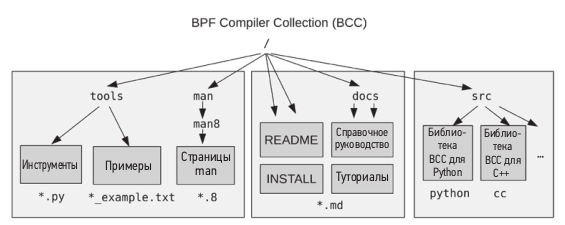
\includegraphics[width=0.8\linewidth]{structure_bcc.png}

\subsection{Схема bpftrace}
\url{https://github.com/bpftrace/bpftrace}

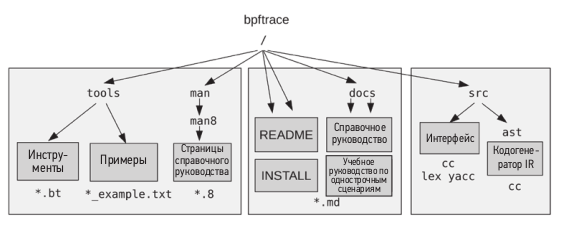
\includegraphics[width=1.0\linewidth]{structure_bpftrace.png}

\subsection{Полезные ссылки}

\noindent BPF Performance Tools - Материалы из книги Brendan Gregg: \\
\indent \url{https://github.com/brendangregg/bpf-perf-tools-book/tree/master} \\

\noindent Docs от разработчиков Bpftrace: \\
\indent \url{https://github.com/bpftrace/bpftrace/tree/master/docs} \\

\noindent BPF на сайте Brendan Gregg: \\
\indent \url{https://brendangregg.com/ebpf.html} \\

\noindent Статья на хабре: \\
\indent \url{https://habr.com/ru/articles/542560/}


\end{document}
